\chapter{Introduction }
\label{chp:intro}

%\section{Introduction}
%A detailed operating system specification was done in the work of ~\cite{group2}. This documentation was critically reviewed and modifications were done in many places to comply with our new design.
%The major modifications done are the following:
%\begin{itemize}
%\item Addition of 8 Kernel registers and 4 Temporary registers (Refer chapter \ref{chp:registers}).
%
%\item The ready queue data structure in the previous design was replaced with a ready list data structure for simplicity in design and implementation (Refer chapter \ref{chp:process}).
%
%\item The maximum number of processes supported by the Operating System was reduced to 12 from 16 due to space constraints in memory (Refer chapter \ref{chp:process}
%
%\item Interrupt specifications were modified due to the size constratits of interrupt code (Refer chapter \ref{chp:int}).
%
%\item The memory layout was modified to incorporate the new design decisions (Refer chapter \ref{chp:memory}).
%\end{itemize}

\section{Brief Machine Description}
\index{Machine}
The machine simulator is known as Extended Simple Integer Machine (\ESIM).
It is an interrupt driven uniprocessor machine.

\section{Components of the Machine}
\index{Machine!Components}
\begin{figure}[ht!]
	\centering
	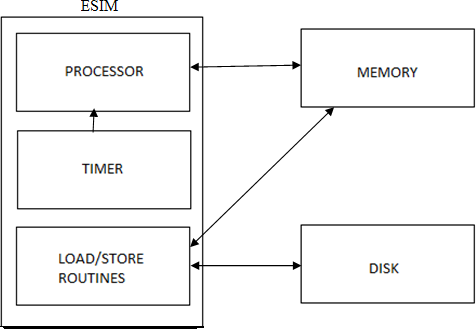
\includegraphics[scale=0.5]{pics/components_machine}
	\caption{Components of the Machine}
	\label{fig:components}
\end{figure}

The various components of the machine are :
\begin{itemize}
	\item \textbf{Disk :} It is a non-volatile storage that stores user programs (executables) and data files. \index{Disk}
	\item \textbf{Memory :} It is a volatile storage that stores the programs to be run on the machine as well as the operating system that manages the various programs. \index{Memory}
	\item \textbf{Processor :} It is the main computational unit that is used to execute the instructions. \index{Processor}
	\item \textbf{Timer :} It is a device that interrupts the processor after a pre-defined specific time interval. \index{Timer}
	\item \textbf{Load/Store :} It is a macro that performs the functionalities of \emph{DMA controller} \index{Load/Store}
	\footnote{\textbf{DMA controller :} DMA (Direct Memory Access) is the hardware device in a real machine that facilitates the transfer of data from disk to the memory and vice versa}.
	% No console device i,e. input output is done through keyboard, monitor and they are not simulated.
\end{itemize}

\section{Data types}
The fundamental types supported by the machine are \textit{integer} and \textit{string}.
\index{Machine!Data Types}
A string is a sequence of characters terminated by \verb|'\0'|. The machine interprets a single character also as a string.
\begin{example}
	The character ``s'' is stored as ``s\verb|\0|'' in the memory and the word ``ESIM'' is stored as ``ESIM\verb|\0|'' in the memory.
\end{example}
\ESIM supports a maximum string length of \emph{16}.
